\section{Introduction}
\label{partIntroduction}

Injuries that occur after a non-penetrating ballistic projectile impacts a Soldier wearing personal protective equipment (PPE) are referred to as behind armor blunt trauma (BABT).  The kinetic energy from such an impact is absorbed by the Soldier's PPE and the bony and soft tissues of the Soldier beneath \cite{Cannon01,grimal2004,cronin2015}.  Standards have been written to which PPE have been designed since 1972.  Verification is through experiments where, typically, a suit of body armor is placed over a ``body'' subjected to a ballistic impact from a projectile fired by a weapon, all in accordance with a standard.  Current practice is to use clay (usually Roma Plastilina No.~1 clay) as a surrogate for the human body in these tests \cite{HanlonGillich2012}.   Injuries that occur from a rapidly increasing overpressure (e.g., shockwaves from an explosion) are denoted as primary blast injuries (PBI) \cite{gibbons2015}.   Blast lung injury (BLI) refers to PBI experienced by the lung \cite{zhou2010}.  Dynamic blunt thoracic trauma can also occur in nonmilitary settings (e.g., automobile accidents), and PBI likewise may occur irrespective of the presence of PPE.

A principal objective of an internal US Army Combat Capabilities Development Command (DEVCOM) Army Research Laboratory (ARL)--Weapons and Materials Research Directorate (WMRD) project, \textit{Modeling Large Deformations and Stress Wave Mechanics in Soft Biological Tissue}, is to develop accurate material models for the human body that are also efficient in their finite element implementation, thereby facilitating the study of BABT and PBI in an effort to improve the designs of PPE.  This is a 6.1 research project whose hand-off to a 6.2 development team at project's end will aid Army engineers in their design of improved PPE by allowing them to run in-silico BABT tests to complement their actual in-field testing.

The DEVCOM Army Research Laboratory-WMRD \textit{Modeling Large Deformations and Stress Wave Mechanics in Soft Biological Tissue\/} project has three primary objectives: \textit{i\/}) new material models, \textit{ii\/}) new experiments, and \textit{iii\/}) new trauma metrics.  Lung has been selected as the soft tissue of interest for this study.  What are sought are models and metrics whose parameters are physical and unique, and whose numeric implementation will be efficient and stable.  Continuum thermo\-dynamic models for lung tissue and a trauma metric are being developed (Clayton, Freed, and co-authors \cite{Clayton2019TRL,ClaytonFreed19,ClaytonFreed20,ClaytonFreed20a,Clayton2019AIP,claytonBM20,clayton2020TRL} and this document).  The work done under this sub-project, \textit{A Dodecahedral Model for Alveoli}, complements its parent project, \textit{Modeling Large Deformations and Stress Wave Mechanics in Soft Biological Tissue}, with regard to the first and third objectives of this ARL-WMRD program.  The models being developed are expected to be improvements over those currently supplied by \texttt{LS-DYNA} in their materials library that, e.g., have been used to study shock waves traversing a human torso not wearing body armor, cf.\ Fig.~\ref{figShockWaveInLung}.  

\begin{figure}
    \centering
    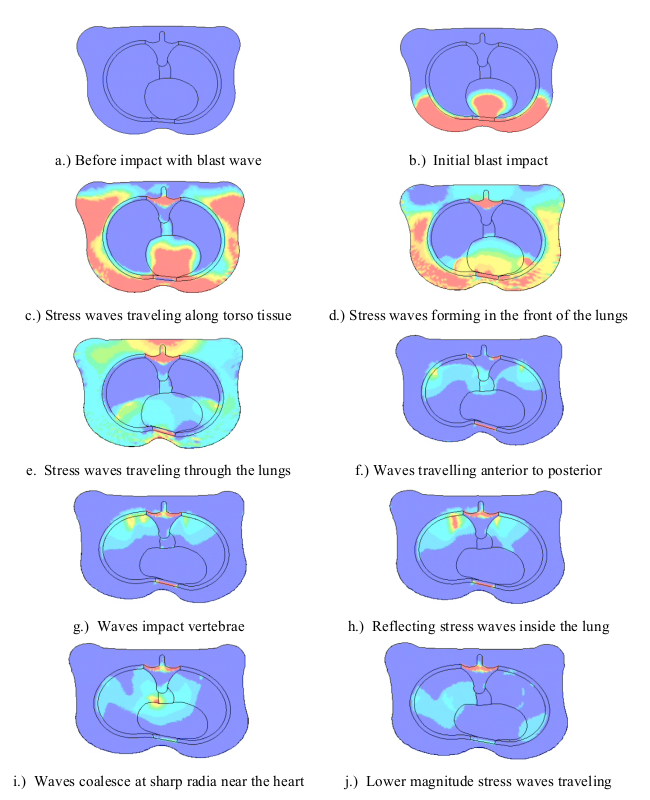
\includegraphics[width=0.95\textwidth]{figures/shockWaveInTorso.png}
    \caption{Finite element analysis done using \texttt{LS-DYNA}  to model shock waves traversing a cross-sectional slice of a human torso.  Material models from the \texttt{LS-DYNA}  library of available models were used \cite{Josey10}.}
    \label{figShockWaveInLung}
\end{figure}

BABT and BLI manifest at the microscopic level of alveoli, which make up the parenchyma, i.e., the spongy tissue of lung that composes around 90\% of lung by volume, cf.\ Fig.~\ref{figLungDrawing}, there being some 500 million alveoli in a typical human lung.  Most damage occurs just beneath the visceral pleural, as seen in Fig.~\ref{figDamagedLung}, and is thought to be a consequence of the large disparity in wave speeds between solid tissues ($\sim$1,500~m/s) and the spongy parenchyma ($\sim$30--40~m/s) \cite{Stuhmiller08}.  The objective of this work is to develop a mechanistic multi-scale model that is capable of describing the deformation and damage that occur at an alveolar level, caused by a shock wave traveling through the parenchyma, induced through either a blast or a ballistic impact to a Soldier's PPE.  In-silico experiments done using this microscopic model are to be used to ``inform'' our macroscopic model in those areas where actual lung experiments are difficult, if not impossible, to perform.

\begin{figure}
    \centering
    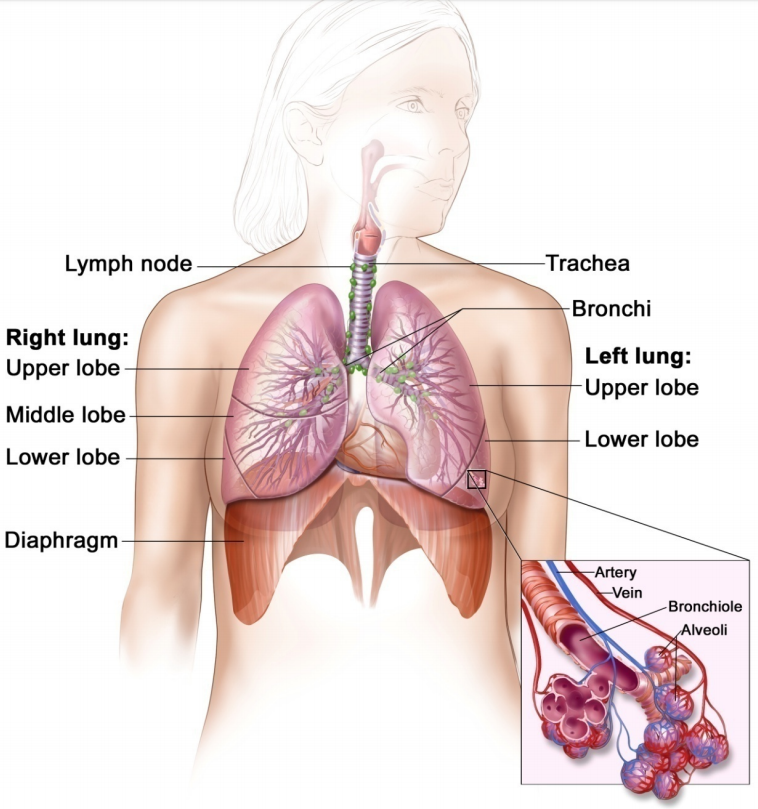
\includegraphics[width=0.7\textwidth]{figures/theRespiratorySystem.png}
    \caption{A medical drawing of the respiratory system \cite{Josey10}}
    \label{figLungDrawing}
\end{figure}

\begin{figure}
    \centering
    \includegraphics[width=0.7\textwidth]{figures/lungInjuryResultingFromBlast.png}
    \caption{Lungs excised from animals (most likely ovine) who expired from blast injury \cite{Stuhmiller08}}
    \label{figDamagedLung}
\end{figure} 

This is the first full-length report for the project \textit{A Dodecahedral Model for Alveoli}.  This first report discusses theoretical foundations and numerical techniques for interrogating the dodecahedral response.  A second report describing results of numerical calculations is anticipated in the next 12 months.

\subsection{$\,$Problem Statement}

Pulmonary contusion is one of the most common thoracic soft-tissue injuries caused by blunt trauma, with a mortality rate of 10\%--25\% \cite{Stitzeletal05}.  Damage to lungs is the main cause of morbidity following high-level blast exposures \cite{Stuhmilleretal88}.  Lung laceration is also common and debilitating \cite{VlessisTrunkey97}.  Existing constitutive models for lung tissue have been developed from limited static test data, e.g., Fung, Vawter \textit{et~al}.\ \cite{Fungetal78,Vawteretal79,Vawter80} These models, and others developed since then, omit relevant physics pertinent to blast and ballistic impacts required to assess BLI and BABT, respectively.  They also require cumbersome optimization protocols to fit non-unique parameter sets \cite{Gayziketal07,Gayziketal11}, and\slash or are not validated against independent data \cite{Yuenetal08}.  Better lung models suitable for dynamic analysis are needed so that the Army can design improved PPE to better protect Soldiers.

The primary objective of the ARL-WMRD project \textit{Modeling Large Deformations and Stress Wave Mechanics in Soft Biological Tissue\/} is to develop such models for deformation and damage\slash injury assessment.  These are continuum models derived from thermo\-dynamics that utilize internal state variables to account for the irreversible aspects of response \cite{ClaytonFreed19,ClaytonFreed20}.  Models (both macro\-scopic and micro\-scopic) are specifically sought whose parameters are physical and whose parameterization is straightforward.  Characterization of the parameters in a model requires experimental data.  This presents an enormous challenge, one that is being addressed in this ARL-WMRD project through other university collaborators.  

Performing experiments for the purpose of model characterization is extremely difficult when it comes to modeling lung.  Lung is a structure; parenchyma is a material.  Therefore, one would normally choose to test the parenchyma, and from these data extract one's model parameters but, because of its spongy nature, we are challenged to do so in a physically meaningful way.  Consequently, one typically tests whole lungs, or lobes thereof, and from these structural experiments we are tasked to extract material parameters through an inverse analysis.  An alternative approach whereby one could, in principle, acquire parameters for the continuum models being developed at ARL-WMRD would be to homo\-genize a microscopic structural response for the alveoli of the parenchyma.  The work presented here addresses this approach in our modeling of deformation, damage, and injury in alveolar structures.

Our approach is also advantageous for understanding the influence of microstructure on the higher-scale continuum properties.  Curve fitting to macroscopic data alone does not provide such insight.  This multi-scale approach can also be used to determine properties for regimes (stress\slash strain\slash strain-rate histories) that cannot be reached experimentally, due to limitations in testing facilities, capabilities, or sufficient animal\slash human tissue availability. 

The narrative that follows seeks to develop two material models for lung: one for mechanical deformation and the other for damage\slash injury\slash trauma.  Models are sought whose parameters have physical interpretation.  Ideally, they will enhance our understanding of the deformation and damage mechanisms at play during BABT and BLI.  Specifically, they will describe how alveoli respond to pressure-waves and\slash or shear-waves as these wave fronts pass through them.  This modeling will be accomplished by constructing a multi-scale model connecting the parenchyma (macro) and alveolar (micro) levels.  In-silico experiments can then be done on the alveolar structural model, whose homogenized response can serve as an aid in the characterization of ARL's continuum models.  These ARL-WMRD continuum models are being designed to perform efficiently in their implementation in finite element codes.  This will allow for BABT and BLI analyses to be done during the design of future PPE with an ultimate goal of saving Soldiers' lives.

The primary purpose of this work is to provide a micro\-scopic model for lung tissue that can be used as an aid in the parameterization of a macro\-scopic model for lung that will be reasonably accurate yet efficient to run in full torso finite element analyses \cite{clayton2020TRL} to study BABT and BLI for the purpose of improving PPE.  Secondarily, the alveolar-level model will provide stand-alone information that will increase our fundamental understanding of the thermomechanical response of lung parenchyma to dynamic loading.  

\subsection{$\,$Approach}

Figure~\ref{figRatLung} shows micrographs from a rat lung taken at different magnifications. In the lower-resolution image, one sees numerous alveoli that became exposed because of the sectioning process.  Also present are several alveolar ducts that connect individual alveoli to a bronchial tree.  In the higher-resolution image we observe the faceted structure of these alveoli, wherein one can see the septal chords and membranes, the latter being traversed by capillaries through which gas exchange occurs.  Gas exchange is not modeled here.

\begin{figure}
    \centering
    \subfigure[Magnification at 100X. This is Fig.~5 in Freed \textit{et~al}.\ \cite{Freedetal12}.]{
        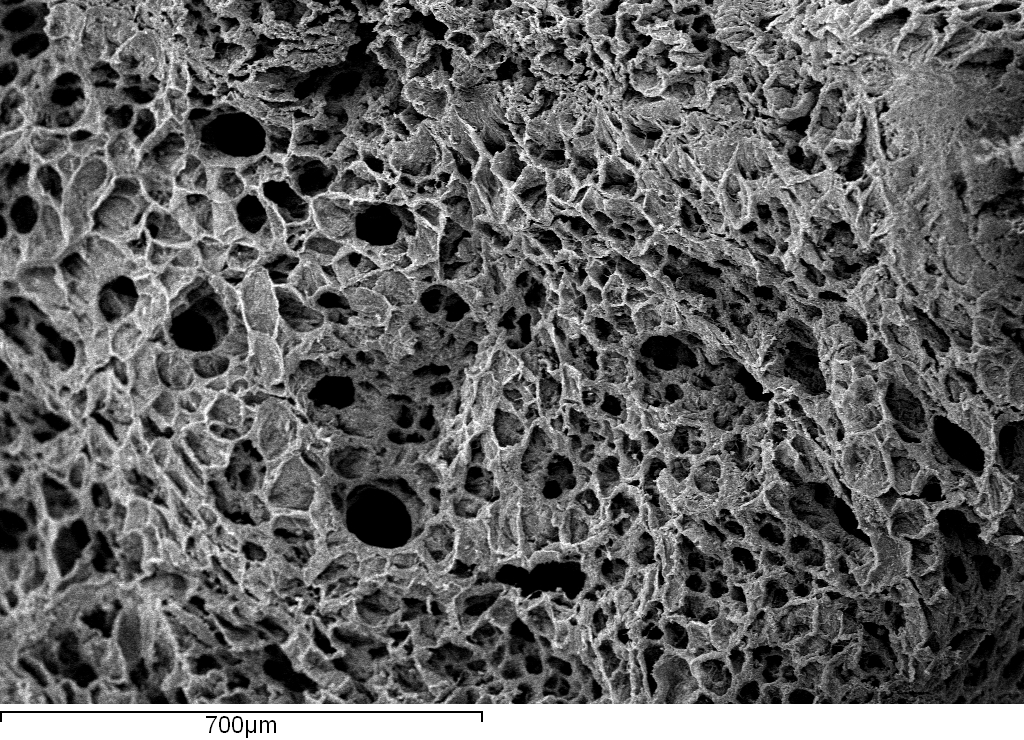
\includegraphics[width=0.45\textwidth]{figures/ratLung100X.jpg}
        \label{figRatLung100}
    }
    \hfill
    \subfigure[Magnification at 750X. This is Fig.~7 in Freed \textit{et~al}.\ \cite{Freedetal12}.]{
        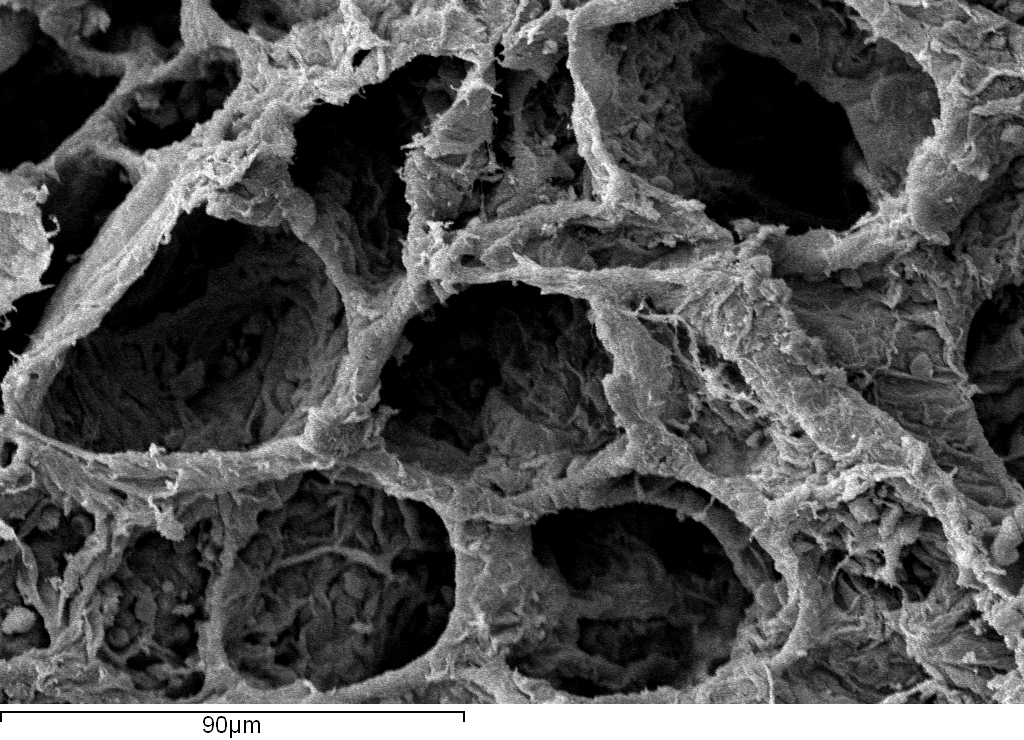
\includegraphics[width=0.45\textwidth]{figures/ratLung750X.jpg}
        \label{figRatLung750}
    }
    \caption{Scanning electron microscopy photographs from a sectioned rat lung.  The alveolar diameter in rat lung is about one quarter the alveolar diameter in human lung.}
    \label{figRatLung}
\end{figure}

Alveolar geometry is modeled here as a dodecahedron, i.e., a soccer-ball like structure comprising 12 pentagonal facets bordered by 30 septal cords that are connected at 20 vertices.  Each vertex links three neighboring cords of the alveolus with a fourth chord from a neighboring alveolus.  BABT and BLI can occur through multiple mechanisms, e.g., tearing of septal cords and\slash or alveolar membranes, and in more severe cases, rupturing of capillaries can also happen causing interstitial fluids and blood to leak into neighboring alveoli, all illustrated in Fig.~\ref{figAlveolarDamage}.  Our dodecahedral model for alveoli is capable of capturing these trauma events.

\begin{figure}
    \centering
    \subfigure[Immunohistochemical staining for hemoglobin showing edema fluid buildups (arrows) caused by blast injury.]{
        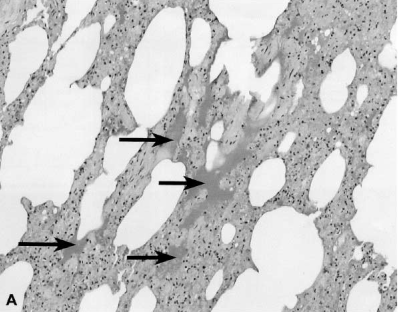
\includegraphics[width=0.3\textwidth]{figures/edemaDamage.png}
        \label{figAlveolarDamageA}
    }
    \hfill
    \subfigure[Histopathology image showing tearing of septal membranes (arrows) caused by blast injury.]{
        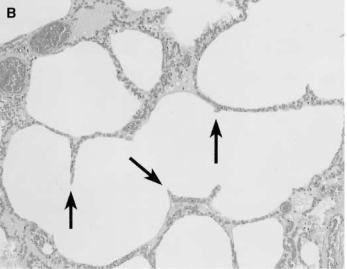
\includegraphics[width=0.3\textwidth]{figures/septalDamage.png}
        \label{figAlveolarDamageB}
    }
    \hfill
    \subfigure[Electron microscope image showing perforations (arrows) of the alveolar wall caused by blast injury.]{
    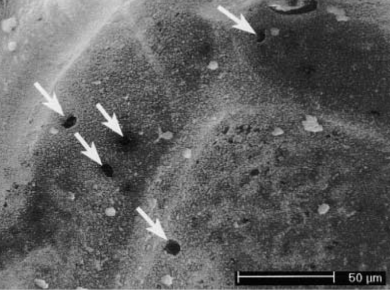
\includegraphics[width=0.3\textwidth]{figures/alveolarDamage.png}
    \label{figAlveolarDamageC}
    }
    \caption{Local injury mechanisms in blast lung. All images from Tsokos \textit{et~al}.\ \cite{Tsokosetal03}.}
    \label{figAlveolarDamage}
\end{figure}

\begin{conj}
\textit{A micro\-scopic strain field, measured at the scale of alveoli, is the same as its macro\-scopic strain field in which it resides, measured at the scale of parenchyma.  The motion is affine, and the local motion is homogeneous.}  
\label{conjecture}
\end{conj}

This hypothesis was tested and confirmed in an experimental study done by Butler \textit{et~al}.\ \cite{Butleretal96} where they used light scattering to study changes in geometry of the septal planes in alveoli, from which they concluded: ``the micro\-scopic strain field does not differ significantly from the macro\-scopic field.''  We employ this hypothesis by taking the deformation gradient from, say, a Gauss point in a finite element model of lung, e.g., from a Gauss point associated with Fig.~\ref{figShockWaveInLung}, and imposing it as a far-field deformation onto our dodecahedral model of an alveolus.  From this kinematic input we arrive at an upper bound on the macro\-scopic stress\slash stiffness response, akin to a Voigt approximation \cite{nemat1999,clayton2011}, through a homogenization of the micro\-scopic forces created within our structural model for an alveolus.

The authors of a recent review article on alveolar strain finished by writing:
\begin{quotation}
    \noindent\small ``In general, computational mechanics approaches to determine function in a healthy or diseased lung have proven to be useful in explaining or measuring observations that are not captured by imaging modalities. However, for these models to fully explain complex physiological mechanical events, appropriate mechanical properties, boundary conditions, and mechanical loads must be identified. Moreover, validation of such computational models, which is an essential component of any computational mechanics approach, remains to be a challenge in the analysis of soft tissue mechanics.''
    
    \nopagebreak
    \mbox{} \hfill Roan \& Waters \cite{RoanWaters11} (p. L633) \normalsize
\end{quotation}
In this research we set out to develop a constitutive framework for alveolar mechanics, fully cognizant of the aforementioned challenges.  Our objectives are different from those of prior studies in alveolar mechanics in that we seek to describe the response\slash injury of a human lung that has been subjected to a stress wave propagating across the thorax region caused by an impact from either a blunt object or a blast wave.  Consequently, some important aspects in the modeling of a breathing lung are thought to be less impactful here, e.g., the effect of surfactant in keeping alveoli from collapsing at the end of expiration.

As a foundation, we adopt the guideline:
\begin{quotation}
	\noindent\small ``Constitutive equations are phenomenological. They are regarded as empirical by experimenters, and axiomatic by mathematicians.  In biomechanics, we often try to derive them on the basis of micro\-structure $\ldots$ in order to gain a better understanding, or to get some guidance to the mathematical form.''
	
	\nopagebreak
	\mbox{} \hfill Y.-C.~Fung \cite{Fung90} (p.~431) \normalsize
\end{quotation}
The approach adopted here is to use the geometry of a dodecahedron as a \textit{micro}\-scopic mechanical model for alveoli, whose far-field response to mechanical stimuli, in accordance with our Conjecture on p.~\pageref{conjecture}, will be used to inform the development of a \textit{macro\/}scopic mechanical model for parenchyma, \cite{ClaytonFreed20} the predominant tissue in lung.  This is deemed necessary because of the complex porous structure of parenchyma, as compared with the homo\-geneous structure of rubbery elastic solids whose theories have historically been employed to model parenchyma \cite{Fung75,Fungetal78,Vawteretal79,Fung88}.  The complementary continuum (macroscopic) model for parenchyma \cite{Clayton2019TRL,ClaytonFreed20,Clayton2019AIP,claytonBM20,clayton2020TRL} is implemented into finite element codes with an end objective of providing a numerical tool that can be used by Army engineers in their efforts to develop improved and more effective designs for a Soldier's PPE. 

\subsection{$\,$Organization}

This document is organized in the following manner.  Section~\ref{partDodecahedron} introduces the dodecahedron as a model for alveoli.  Its geometric properties are derived in detail with regards to its three geometric features: 1D septal chords, 2D septal membranes, and 3D alveolar sacs.  Section~\ref{partKinematics} develops the kinematics required for us to model a deforming dodecahedron, again focusing on the 1D~chords, 2D~membranes, and the 3D~volume within, including the shape functions needed for interpolating each geometry.  Section~\ref{partConstitutive} derives constitutive models suitable for describing the thermomechanical response for the structural constituents of an alveolus: its septal chords, its permeable membranes, and its volume.  Section~\ref{partNumericalMethods} presents numerical methods used for solving first- and second-order, ordinary, differential equations (ODEs) and spatial integrations along a bar, across a pentagon, and throughout a tetrahedron using Gaussian quadrature schemes designed for each geometry.  Section~\ref{partVariational} describes a variational formulation used to create our structural modeling of an alveolus, which consists of three separate models: one consisting of septal chords, another consisting of septal membranes, and the third consisting of alveolar volume.  Forces at the vertices are summed and homogenized for return to the macroscopic solver.  Constitutive equations suitable for modeling biological tissues are derived from thermo\-dynamics using the theory of implicit elasticity, and are presented in the Appendix.
